\chapter{Turbomeet}
\label{Turbomeet}

Turbomeet ist der Prototyp an dem verschiedene Libraries und Tools getestet werden. Es ist eine Webseite auf der sich Nutzer anmelden können und Meetings mit verschiedenen Zeitslots erstellen können. Für diese Zeitslots kann dann von anderen Nutzern abgestimmt werden. Wenn ein Meeting abgeschlossen wird bzw. die Deadline erreicht wird, werden die Zeitslots mit den meisten Teilnahmen ausgewählt.

\section{Technologien}
\label{Technologies}

Der ausgewählte Technologie Stack ist der T3-Stack:

\begin{itemize}
    \item Next.js
    \item TypeScript
    \item tRPC
    \item TailwindCSS
    \item Prisma
    \item NextAuth.js
\end{itemize}

Neben diesen Technologien werden noch weitere Libraries verwendet, die in den folgenden Abschnitten genauer beschrieben werden.

\subsection{Next.js}

Next.js ist ein serverseitiges JavaScript-Framework, das auf React aufbaut. Es ist dafür ausgelegt, schnelle und skalierbare Anwendungen zu entwickeln. Zu den Funktionen von Next.js gehören:

\begin{itemize}
    \item Serverseitiges Rendern (SSR): Next.js kann die HTML-Ausgabe auf dem Server generieren, was die Ladezeit der Seite verbessert und die Suchmaschinenoptimierung (SEO) erleichtert.
    \item Automatisches Code-Splitting: Next.js teilt automatisch den Code in kleine, optimierte Teile auf, um die Ladezeit der Seite zu reduzieren.
    \item Hot-Module-Replacement: Next.js aktualisiert automatisch den Code, während Sie arbeiten, um einen schnellen Entwicklungsprozess zu ermöglichen.
    \item Static Site Generation (SSG): Next.js kann auch statische Seiten generieren, um schnelle und sichere Websites zu erstellen, die auf einem CDN (Content Delivery Network) gehostet werden können.
\end{itemize}

\subsection{TypeScript}

TypeScript ist eine freie und quelloffene Programmiersprache, die auf JavaScript basiert. Sie ist eine statisch typisierte Sprache, die es Entwicklern ermöglicht, die Typen von Variablen und Funktionen zu definieren. Dadurch können Fehler frühzeitig erkannt und behoben werden. Außerdem können Entwickler mit TypeScript auch die neuesten Funktionen von JavaScript verwenden, ohne auf die Kompatibilität mit älteren Browsern achten zu müssen.

\subsection{tRPC}

tRPC ist ein Open-Source-Framework, das es Entwicklern ermöglicht, API Endpunkte einfach zu definieren und zu erstellen. Mit dem Motto \emph{``Move fast and break nothing. End-to-end typesafe APIs made easy.``} (\citeurl{httpstrpcio_trpctrpc_nodate}) werden die Vorteile von tRPC sehr gut beschrieben. Durch die Nutzung von TypeScript im Backend sowie im Frontend werden Breaking Changes vermieden und die Entwicklung wird beschleunigt. Wenn bestimmte Felder z.B. in der API geändert/entfernt werden, und auf diese im Frontend zugegriffen wird, werden diese direkt mit spezifischen Fehlern annotiert.

Um eine E2E Typensicherheit bei normalen REST und GraphQL APIs zu erhalten muss eine Vielzahl von Tools und Konfiguration vorgenommen werden. Dies ist meist sehr aufwändig und komplex.

\subsection{TailwindCSS}

TailwindCSS ist ein Utility-First CSS-Framework. Das bedeutet, dass es keine vorgefertigten Komponenten wie z.B. Buttons oder Formulare gibt. Stattdessen werden die Komponenten aus einzelnen Utility-Klassen zusammengesetzt. Diese Utility-Klassen sind meist sehr spezifisch und beschreiben nur eine Eigenschaft. So kann z.B. ein Button mit der Klasse \texttt{.bg-blue-500} eine blaue Hintergrundfarbe erhalten. Die Klasse \texttt{.bg-blue-500} beschreibt nur die Hintergrundfarbe und nicht die Größe oder den Abstand zum nächsten Element. Diese Utility-Klassen können dann beliebig kombiniert werden, um die Komponente zu gestalten.

\subsection{Prisma}

Prisma ist ein Open-Source-ORM (Object-Relational Mapping) für Node.js. Es ermöglicht es Entwicklern, Datenbanken zu modellieren und mit der Datenbank zu interagieren. Prisma bietet eine einfache und intuitive API, die es Entwicklern ermöglicht, Datenbankabfragen zu schreiben, ohne sich um die Syntax der Datenbank kümmern zu müssen. Prisma unterstützt eine Vielzahl von Datenbanken, darunter MySQL, PostgreSQL, SQLite und MongoDB.

Prisma generiert automatisch eine TypeScript Typen Definition für die Datenbank. Mithilfe dieser Typen Definition können Entwickler sicherstellen, dass die Datenbank und die API Endpunkte immer synchron sind.

\subsection{NextAuth.js}

NextAuth.js ist ein Open-Source-Framework, das es Entwicklern ermöglicht, Authentifizierung und Autorisierung in Next.js Anwendungen zu implementieren. Es bietet eine einfache und intuitive API, die es Entwicklern ermöglicht, verschiedene Authentifizierungsmethoden zu implementieren, wie z.B. OAuth, E-Mail-Authentifizierung, Passwort-Authentifizierung, Magic-Links, etc.

\subsection{Radix UI}

Wie bereits in dem \hyperref[secsec:radix]{Recherche Kapitel} beschrieben ist Radix UI ein \emph{primitive-first} UI-Framework. Es werden z.B. Komponenten wie Buttons, Inputs und Dialoge bereitgestellt. Diese sind immer bereits mit der Funktionalität und Accessability Features ausgestattet. Außerdem sind die Komponenten un-styled, d.h. sie haben keine vorgefertigte CSS-Klasse. Stattdessen können die Komponenten mit den Utility-Klassen von TailwindCSS gestyled werden.

Alle Komponenten von Radix UI folgen dem \emph{WAI-ARIA} Standard und implementieren die Accessability Patterns der \emph{APG} wie in im Kapitel \ref{secsec:apg_patterns} beschrieben. Dadurch werden den Entwicklern bereits viele Accessability Features zur Verfügung gestellt und es muss nicht jedes Mal alles neu/manuell implementiert werden.

Bestimmte Felder wie z.B. die \texttt{label} eines Inputs können mit einem \texttt{aria-label} versehen werden. Dadurch wird der Input für Screenreader und andere Assistive Technologien lesbar. Diese Werte kann Radix UI nicht automatisch generieren, da es nicht weiß, was in den Feldern steht. Deshalb müssen diese Werte manuell angegeben werden. Aber auch hier hilft Radix UI, indem es in der Dokumenation explizit darauf hinweist, dass diese Werte angegeben werden müssen.

In der Dokumenation zu den einzelnen Komponenten werden außerdem die Accessability Features beschrieben. So wird z.B. bei einem Dialog beschrieben, dass der Dialog mit der Tastatur bedienbar ist und wie dies funktioniert. Außerdem wird beschrieben, dass der Dialog mit einem Screenreader gelesen werden kann. In Abbildung \ref{fig:radix_dialog_keyboard} ist ein Screenshot der Dokumenation zu einem Dialog zu sehen.

\begin{figure}[th]
\centering
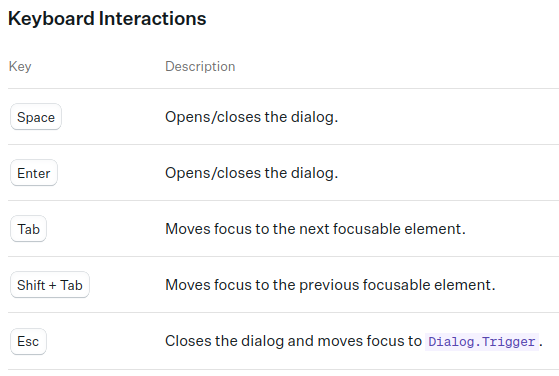
\includegraphics[width=0.75\textwidth]{Figures/radix_dialog_keyboard.png}
\decoRule
\caption[Dialog Accessability Dokumenation]{Radix UI Dialog Accessability Dokumenation}
\label{fig:radix_dialog_keyboard}
\end{figure}

\subsection{CmdK}

CmdK ist eine Open-Source-Library, die eine Komponenten basierte Accessability optimierte \textit{Combobox} bereitstellt. Eine \textit{Combobox} ist eine Kombination aus einem \textit{Input} und einer \textit{Dropdown} Liste. Diese wird inzwischen häufig auf Webseiten/Tools wie GitHub, Linear und TailwindCSS (siehe Abbildungen \ref{fig:cmdk_github}, \ref{fig:cmdk_linear}, \ref{fig:cmdk_tailwindcss}) genutzt um zum einen eine Suchfunktion zu implementieren oder um eine Liste von Aktionen / Optionen anzuzeigen. Die Tastenkombinationen für solche Funktionen sind von System zu System unterschiedlich. Zum Beispiel stellt macOS unter \emph{Cmd + Leertaste} eine Globale Such/Kommandofunktion zur Verfügung auf Webseiten wird meist eher \emph{Cmd + K} (macOs) oder \emph{Ctrl + K} (Windows) verwendet. Eine weitere Variante ist das einfache drücken von ``/``. Dies ist aber z.B. auf dem deutschen QWERTZ-Tastatur Layout nicht direkt möglich.

\begin{figure}[th]
    \centering
    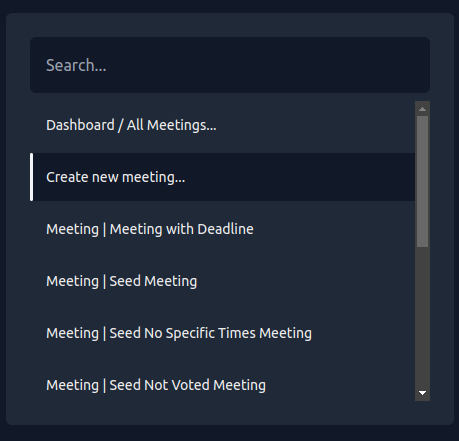
\includegraphics[width=0.6\textwidth]{Figures/turbomeet_cmdk.png}
    \decoRule
    \caption[Turbomeet Kombobox]{Turbomeet Kombobox für Seitennavigation/Suche}
    \label{fig:turbomeet_cmdk}
\end{figure}

Die Implementierung in Turbomeet (siehe Abbildung \ref{fig:turbomeet_cmdk}) lässt quasi alle oben genannten Kombinationen zu um Systemunabhängig für verschiedene Nutzer einfach bedienbar zu sein.

Zur Auswahl stehen unter anderem die Hauptseite wie das Dashboard, Nutzerprofil oder die Datenschutzerklärung, dazu werden außerdem Direkt-Verlinkungen zu den eigenen Meetings mit angezeigt. Des Weiteren werden Funktionen wie das erstellen von neuen Meetings oder das wechseln des Themes direkt ansprechbar gemacht.

Diese Funktionalität ist auch für die Accessability ein sehr interessantes Feature. So kann z.B. ein Screenreader Nutzer die Kombobox öffnen und die verfügbaren Optionen durchlesen. Wenn ein Nutzer eine Seite bereits kennt, kann er durch die Suche direkt zu dieser springen ohne erst durch verschlungene Navigationen und Submenüs zu navigieren. Hierbei sind aber auch wieder die Entwickler gefragt um die Suchbegriffe so zu wählen, dass sie für den Nutzer intuitiv sind. Dies kann z.B. auch durch eine duplizierte Navigation unter verschiedenen Begriffen erreicht werden. Dies wäre in einer normalen Navigation nicht möglich, da die Navigation dann zu unübersichtlich wird.

Ein großer Vorteil von CmdK ist, dass es für die Dialog/Popover Implementierung Radix-UI als Basis nutzt. Dies ist für Turbomeet von Vorteil, da Radix sowieso genutzt und geladen wird und somit keine zusätzlichen Abhängigkeiten hinzugefügt werden müssen und darauf vertraut werden kann, dass die Accessability Features von Radix auch in CmdK implementiert sind.

\section{Analyse}

\subsection{Lighthouse}

Da Lighthouse eines der am einfachsten und schnellsten Tools für eine Analyse auch während der Entwicklung ist habe ich mich vorrangig darauf gestützt. Die Ergebnisse wahren hier auch immer recht gut und ich konnte so schnell die kleinen Dinge verbessern, die noch nicht optimal waren. Die Ergebnisse von einem Zwischenstand sind in der folgenden Abbildung \ref{fig:lighthouse_desktop_1} zu sehen. Die kompletten Berichte sind als PDF verfügbar, aber nicht im Anhang eingebunden, da diese über 100 Seiten umfassen. Daher sind sie über die folgenden Links erreichbar: \href{URL}{text}

\begin{figure}[th]
    \centering
    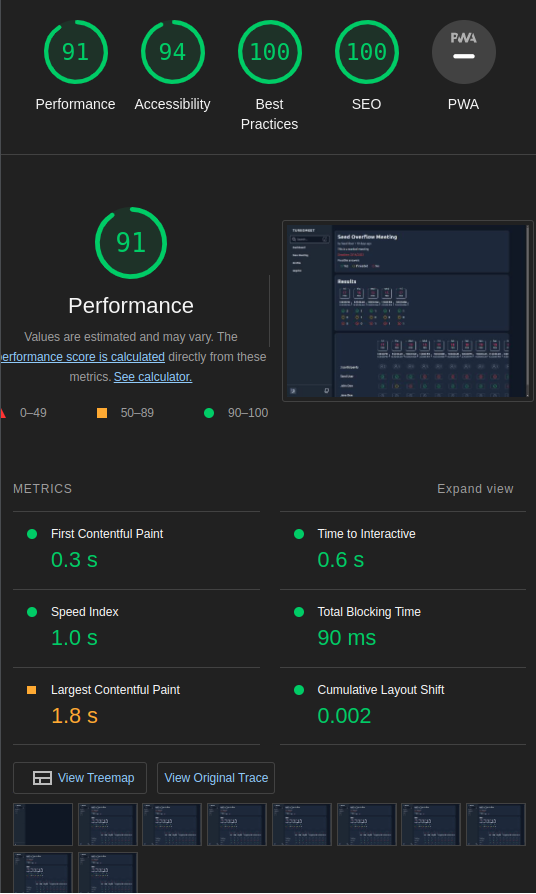
\includegraphics[width=0.45\textwidth]{Figures/lighthouse_desktop_1.png}
    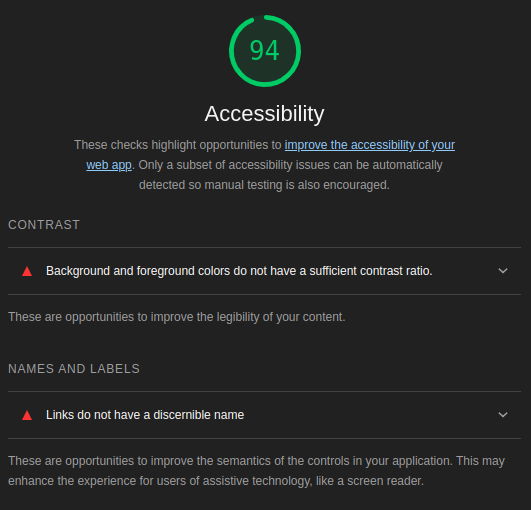
\includegraphics[width=0.45\textwidth]{Figures/lighthouse_desktop_2.png}
    \decoRule
    \caption[Turbomeet Lighthouse Bericht Desktop]{Lighthouse Bericht für Desktop}
    \label{fig:lighthouse_desktop_1}
\end{figure}

Im Bereich Accessability wurde hier z.B. darauf hingewiesen, dass die Hinter- /Vordergrund (Text) Farben zu wenig Kontrast haben und dass bei vielen Links die Beschreibungen fehlen. Als ich dann aber die Analyse noch einmal für das Mobile-Preset durchgeführt habe (siehe Abbildung \ref{fig:lighthouse_mobile_1}) 
sank die Performance von 91\% auf gerade einmal 52\%, die TTI (Time to Interactive) von 0.6s auf 6.7s und die LCP (Largest Contentful Paint) von 1.8s auf 9.2s.

\begin{figure}[th]
    \centering
    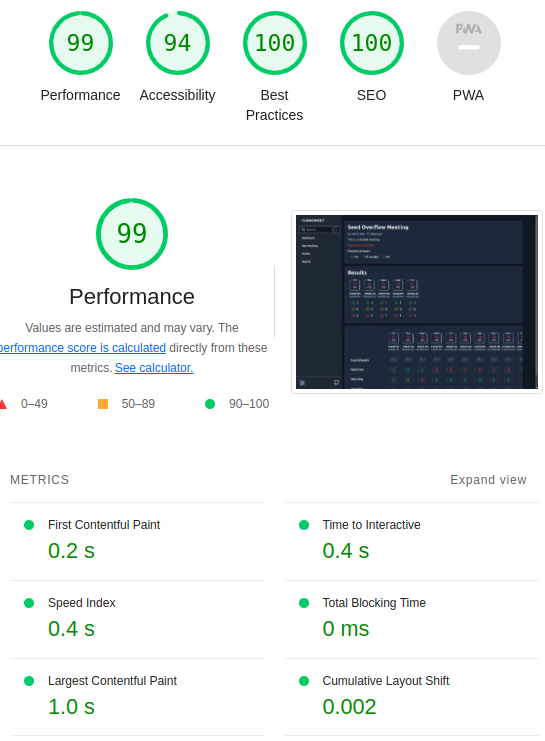
\includegraphics[width=0.45\textwidth]{Figures/lighthouse_desktop_4.png}
    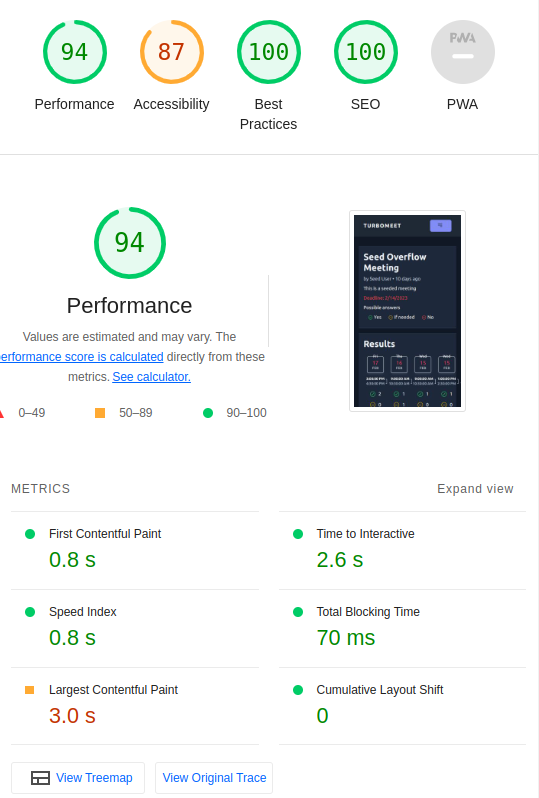
\includegraphics[width=0.45\textwidth]{Figures/lighthouse_mobile_2.png}
    \decoRule
    \caption[Turbomeet Lighthouse Bericht Chromium]{Lighthouse Bericht Chromium (links: Desktop, rechts: Mobile)}
    \label{fig:lighthouse_mobile_2}
\end{figure}

Glücklicherweise gab Lighthouse aber auch direkt den richtigen Tipp, welchen bereits im Kapitel \ref{sec:a11yToolsLighthouse} beschrieben wurde. Durch das Testen in meinem normalen Browser waren verschiedene Erweiterungen aktiv, welche sich in den Render Prozess von React einhängen um so während der Entwicklung States und ähnliche Dinge auszulesen. Aus diesem Grund schlägt Lighhouse hier vor, die Erweiterungen zu deaktivieren oder auf einen Inkognito Modus umzusteigen. Mit einem erneuten Test in einem cleanen Chromium Browser wurde nun wieder eine sehr gute Performance erreicht, jedoch sank die Accessability trotzdem noch auf 87\%. Dies liegt daran, dass Lighthouse in der Mobilen Variante alle Links als Buttons interpretiert und somit die Beschreibungen für die Button (Links) verlangt. Anscheinend weißt Lighthouse diesem dann auch mehr Gewicht zu als in der Desktop Variante. Dies ist aber auch kein Problem, da die Beschreibungen für die Links sowieso noch fehlen und somit schnell nachgeholt werden können.

Daraus lässt sich mitnehmen, immer beide Varianten zu testen, da die Ergebnisse sich unterscheiden können und auch verschiedene Optimierungen für Desktop und Mobile getroffen werden müssen. 

Die Punkte SEO und Best Practices wurden hierbei in beiden Varianten mit 100\% bewertet und dies ohne das extra Aufwände dafür getätigt werden mussten. Dies liegt daran, dass Turbomeet auf einen Technologie Stack aufbaut, welcher zum einen Next.js und das SSR Feature nutzt, wodurch die Seiten bereits vor dem Laden der Seite, auf dem Server, gerendert werden und somit auch schon für Suchmaschinen verfügbar sind (Crawlable für Google Bots). Zum anderen wird TypeScript genutzt, durch welches die neusten Features von JavaScript auch in älteren Browser polyfilled und deprecated APIs vermieden werden und somit eine sehr gute Performance erreicht wird.